%template1.tex
%The following LaTeX source file represents the simplest kind of slide presentation; no overlays, no included graphics. Substitute your favorite style for ``pascal''. To create the PDF file template1.pdf, (1) be sure to use the prosper class, then (2) execute the command latex template1.tex, and (3) the command dvipdf template1.dvi.

%%%%%%%%%%%%%%%%%%%%%%%%%%%%%%% template1.tex %%%%%%%%%%%%%%%%%%%%%%%%%%%%%%%%%%%
\documentclass[a4paper,blends,pdf,colorBG,slideColor]{prosper}
% definitions for slides for CSC544
% Lutz Hamel, (c) 2007

\hypersetup{pdfpagemode=FullScreen}

\usepackage{times}
\usepackage{latexsym}
\usepackage{alltt}
\usepackage{booktabs}
\usepackage{amsmath}
\usepackage{amsopn}
\usepackage{amsfonts}
\usepackage{amssymb}
%\usepackage[usenames]{color}

\def\sign{\qopname\relax{no}{sign}}
\def\argmax{\qopname\relax{no}{argmax}}
\def\argmin{\qopname\relax{no}{argmin}}

\newcommand{\grad}{\ensuremath{\nabla}} 
\newcommand{\loss}{\ensuremath{{\cal L}}}
\newcommand{\err}{\mbox{err}}
\newcommand{\mse}{\mbox{mse}}
\newcommand{\acc}{\mbox{acc}}
\newcommand{\Integer}{\ensuremath{\mathbb{N}}}
\newcommand{\size}[1]{{|{#1}|}}
\newcommand{\Rnspace}[1]{\ensuremath{\mathbb{R}^{#1}}}
\newcommand{\Real}{\ensuremath{\mathbb{R}}}
\newcommand{\mytt}[1]{{\small\tt{#1}}}
\newcommand{\textemph}[1]{{\em #1}}
\newcommand{\suchthat}{\mid}
\newcommand{\orbar}{\;|\;}
\newcommand{\bs}[1]{\begin{slide}{#1}\ptsize{8}}
\newcommand{\es}{\end{slide}}
\newcommand{\co}{\,\colon\;}
\newcommand{\pair}[2]{\ensuremath{( {#1}, {#2} )}}
\newcommand{\model}[1]{\hat{#1}}
\newcommand{\ul}[1]{{\bf\em #1}}
\newcommand{\ol}{\overline}
\newcommand{\definition}[1]{{\bf Definition: }{\em #1}}
\newcommand{\example}[1]{{\bf Example: }{#1}}
\newcommand{\abs}[1]{|{#1}|}
\newcommand{\mytab}{\makebox[.1in]{}}

\newcommand{\fdef}[1]{
\begin{center}
\fbox{
\begin{minipage}{3.5in}
{\bf Definition:}
{#1}
\end{minipage}
}
\end{center}
}

\newcommand{\fframe}[1]{
\begin{center}
\fbox{
\begin{minipage}{3.5in}
{#1}
\end{minipage}
}
\end{center}
}

\newcommand{\nframe}[1]{
\begin{center}
\begin{minipage}{3.5in}
{#1}
\end{minipage}
\end{center}
}

\newenvironment{Rcode}
	{
		\scriptsize
		\begin{quote}
		\begin{alltt}
	}
	{
		\end{alltt}
		\end{quote}
	}




\begin{document}

\bs{Non-Linear SVMs}
\vspace{.2in}
\begin{itemize}
\item
The linearity assumption on the training data is a very strong assumption.

\item
Not many real-world data sets are linearly separable and therefore our current setting is
somewhat unrealistic.

\item
Turns out that the linear setting of SVMs can easily be extended to the non-linear setting
by considering {\em kernel functions}.

\end{itemize}
\es

\bs{A Non-Linear Data Set}
\small
\begin{center}
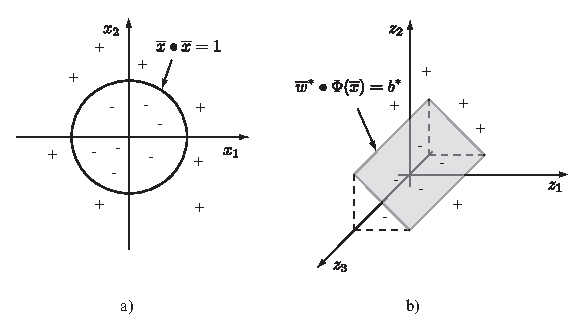
\includegraphics[height=30mm]{figures/fig07-03.eps}
\end{center}
Here the figure a) represents a non-linear data set in our input space $\Rnspace{2}$:
\begin{itemize}
\item
There exists no linear decision surface $\ol{w}\bullet\ol{x}=b$
that would separate this data.
\item
The non-linear decision surface $\ol{x}\bullet\ol{x} = 1$ does separate the data.
\end{itemize}
Now, instead of computing a classification model in the input space, we first map our data set
into a higher dimensional {\em feature space} and then compute the model,
\begin{equation*}
\model{f}(\ol{x}) = \sign \left (\ol{w}\bullet{\color{red}\Phi}(\ol{x}) - b\right),
\end{equation*}
with $\Phi\co \Rnspace{2} \rightarrow \Rnspace{3}$ and
\begin{equation*}
\Phi(\ol{x}) = \Phi(x_1,x_2) = (x_1^2,x_2^2,\sqrt{2}x_1 x_2) .
\end{equation*}
\es

\bs{A Non-Linear Data Set}
\vspace{.2in}
Observations:

\begin{itemize}
\item The mapping $\Phi$ maps our 2-D input space into a 3-D feature space.
\item The mapping $\Phi$ converts our non-linear classification problem into a linear classification 
problem.
\item It can be shown that all the points within the circle in input space are below the linear
decision surface in feature space and all the points outside of the circle in input space
are above the linear decision surface in feature space.

\item We have just constructed a {\em non-linear decision function}!
\end{itemize}
\es

\bs{A Non-Linear Decision Function}
Given our data set and $\Phi$ we can construct a decision function
that separates the non-linear data set,
\begin{equation*}
\model{f}(\ol{x}) = \sign\left ( \ol{w}^*\bullet\Phi(\ol{x}) - b^* \right).
\end{equation*}
with $\ol{w}^*=  (w^*_1, w^*_2, w^*_3) = (1,1,0)$ and $b^* = 1$. 

It is perhaps revealing to study this decision function in more detail,
\begin{equation*}
\begin{aligned}
\model{f}(\ol{x}) 
	& =  \sign\left (\ol{w}^*\bullet\Phi(\ol{x}) - b^*\right )\\
	& =  \sign\left (w^*_1 x_1^2 + w^*_2 x_2^2 + w^*_3 \sqrt{2} x_1 x_2 - b^*\right )\\
	& =  \sign\left (\sum_{i=1}^{\color{red}3} w^*_i z_i - b^*\right ),
\end{aligned}
\end{equation*}
where $\Phi(\ol{x}) = \Phi(x_1,x_2) = (z_1,z_2,z_3) = \ol{z}$.

We obtain a decision surface in feature space whose complexity depends
on the number of dimensions of the feature space.

\es

\bs{A Non-Linear Decision Function}
\small
We can expect that the more complex the non-linear decision surface is in the input space, the more
complex the linear decision surface in feature space (the larger $d$),

\begin{equation*}
\model{f}(\ol{x}) =  \sign\left (\sum_{i=1}^{\color{red}d} w^*_i z_i - b^*\right ).
\end{equation*}
But, now consider the dual representation of $\ol{w}^*$,
\begin{equation*}
\ol{w}^* = \sum_{i=1}^l \alpha^*_i y_i  \Phi(\ol{x}_i),
\end{equation*}
then,
\begin{align*}
\model{f}(\ol{x}) &=  \sign\left ({\color{red}\sum_{i=1}^d} w^*_i z_i - b^*\right )\\
&=  \sign\left (\ol{w}^*\bullet \ol{z} - b^*\right )\\
&=  \sign\left (\ol{w}^*\bullet\Phi(\ol{x})  - b^*\right )\\
&=  \sign\left ({\color{red}\sum_{i=1}^l} \alpha^*_i y_i  \Phi(\ol{x}_i)\bullet\Phi(\ol{x})  - b^*\right ).
\end{align*}

\es

\bs{Kernel Functions}
Observations:

\begin{itemize}
\item We have reduced the problem from a problem in terms of feature space dimensionality
to a problem that depends on the number of support vectors.

\item Functions of the form $\Phi(\ol{x})\bullet\Phi(\ol{y}) $ are called kernel functions.

\item In our particular case we have $\Phi(\ol{x})\bullet\Phi(\ol{y}) = (\ol{x}\bullet\ol{y})^2$, that is
the computation in feature space reduces to a computation in input space.  (convince yourself of this)

\end{itemize}
\es

\bs{Kernel Functions}
\small
If we let $k(\ol{x},\ol{y}) =\Phi(\ol{x})\bullet\Phi(\ol{y}) $ be a kernel function, then we can write
our support vector machine in terms of kernels,
\begin{align*}
\model{f}(\ol{x}) &=  \sign\left (\sum_{i=1}^l \alpha^*_i y_i  \Phi(\ol{x}_i)\bullet\Phi(\ol{x})  - b^*\right )\\
	&=  \sign\left (\sum_{i=1}^l \alpha^*_i y_i  {\color{red}k(\ol{x}_i,\ol{x})}  - b^*\right )
\end{align*}
We can apply the same kind of reasoning to $b^*$ which is the offset term in feature space,
\begin{align*}
b^* & = \sum_{i=1}^l \alpha^*_i y_i  \Phi(\ol{x}_i)\bullet\Phi(\ol{x}_{sv^+}) - 1\\
	& = \sum_{i=1}^l \alpha^*_i y_i  {\color{red}k(\ol{x}_i,\ol{x}_{sv^+})} - 1
\end{align*}
This means, that the support vector machine in feature space is completely determined by
the support vectors and an appropriate kernel function.

The fact that we are free to choose any kernel function for our model is called the {\color{red}{\em kernel trick}}.
\es

\bs{Kernel Functions}
\begin{tabular*}{\textwidth}{@{\vrule height 16pt depth 4pt width 0pt \hskip\arraycolsep\extracolsep{\fill}}l l l}
      \toprule
Kernel Name & Kernel Function & Free Parameters \\
      \midrule
Linear Kernel & 
	$k(\ol{x},\ol{y}) = \ol{x} \bullet \ol{y} $ & 
		none \\ 
Homogeneous Polynomial Kernel & 
	$k(\ol{x},\ol{y}) = (\ol{x} \bullet \ol{y})^d$ & 
		$d \geq 2$ \\ 
Non-Homogeneous Polynomial Kernel & 
	$k(\ol{x},\ol{y}) = (\ol{x} \bullet \ol{y} + c)^d$ & 
		$d \geq 2$, $c > 0$ \\ 
Gaussian Kernel & 
	$k(\ol{x},\ol{y}) = e^{-\frac{\abs{\ol{x}-\ol{y}}^2}{2\sigma^2}}$ & 
		$\sigma > 0$ \\ 
      \bottomrule
   \end{tabular*}
\es



\end{document}
%%%%%%%%%%%%%%%%%%%%%%%%%%% end of template1.tex %%%%%%%%%%%%%%%%%%%%%%%%%%%%%%%%

